% Slide thuyết trình — biên dịch: cd report && latexmk -xelatex slides.tex
\documentclass[aspectratio=169,11pt]{beamer}
\usetheme{metropolis}
\usepackage{fontspec}
\setsansfont{texgyreheros}[Extension=.otf,UprightFont=*-regular,BoldFont=*-bold,ItalicFont=*-italic,BoldItalicFont=*-bolditalic]
\setmonofont{texgyrecursor}[Extension=.otf,UprightFont=*-regular,BoldFont=*-bold,Scale=0.95]
\usepackage[vietnamese]{babel}
\usepackage{booktabs,graphicx,tikz}
\usetikzlibrary{positioning,arrows.meta}
\graphicspath{{../outputs/final/figures/}}
\newcommand{\code}[1]{\texttt{#1}}
\setbeamertemplate{frame footer}{RNN/CNN cho phát hiện ransomware --- BitcoinHeist}
\setbeamerfont{footnote}{size=\tiny}

\title{Phát hiện ransomware trên chuỗi khối Bitcoin\\bằng LSTM/GRU và CNN}
\subtitle{Đồ án cuối kỳ --- Nhập môn Học máy}
\author{Nhóm: [Họ tên thành viên --- MSSV]}
\date{}

\begin{document}
\maketitle

\begin{frame}{Bài toán và dữ liệu}
\begin{columns}[T]
\column{0.55\textwidth}
\begin{itemize}
\item \textbf{BitcoinHeist}: 2,9 triệu dòng = (địa chỉ, ngày), 6 đặc trưng đồ thị giao dịch + năm, ngày.
\item \textbf{7 lớp}: \code{white} + 5 họ ransomware lớn + \code{otherRansom}.
\item \textbf{Mất cân bằng nặng}: \code{white} 98,6\%; lớp nhỏ nhất 1.441 dòng\\ $\Rightarrow$ độ đo chính: \textbf{macro F1}.
\item Dữ liệu \textbf{dạng bảng} --- không phải ảnh/văn bản/chuỗi thời gian.
\end{itemize}
\column{0.42\textwidth}
\small
\begin{tabular}{lr}
\toprule
Lớp & Số dòng \\
\midrule
white & 2.875.284 \\
CryptoWall & 12.390 \\
CryptoLocker & 9.315 \\
Cerber & 9.223 \\
Locky & 6.625 \\
CryptXXX & 2.419 \\
otherRansom & 1.441 \\
\bottomrule
\end{tabular}
\end{columns}
\end{frame}

\begin{frame}{Quan sát then chốt: địa chỉ được dùng lại}
\begin{itemize}
\item CryptoLocker, CryptoWall, otherRansom: chỉ \textbf{15--23\%} dòng là lần đầu địa chỉ xuất hiện
  (1.894 địa chỉ CryptoWall $\to$ 12.390 dòng).
\item Cerber, Locky: \textbf{99,5\%} dòng là lần đầu --- mỗi nạn nhân một địa chỉ mới.
\item Chia ngẫu nhiên (như Bài 1): 54,7\% dòng ransomware trong test có địa chỉ đã gặp ở train $\Rightarrow$ cần
  \textbf{chia theo địa chỉ} khi dùng lịch sử.
\end{itemize}
\vspace{4pt}
\alert{$\Rightarrow$ Lịch sử của một địa chỉ là một chuỗi thời gian thật --- chỗ cho RNN/CNN phát huy.}
\end{frame}

\begin{frame}{Hai cách biến dòng dữ liệu bảng thành chuỗi}
\begin{columns}[T]
\column{0.48\textwidth}
\textbf{A --- mỗi đặc trưng là một bước}
\begin{itemize}\small
\item 11 đặc trưng số (6 gốc + 5 tạo thêm), log1p + chuẩn hoá.
\item Token hoá: $\mathbf{e}_i = x_i\mathbf{W}_i + \mathbf{b}_i \in \mathbb{R}^{16}$ $\to$ chuỗi $11\times16$.
\item Chia ngẫu nhiên phân tầng 64/16/20 --- \textbf{giống Bài 1}.
\item Hạn chế: thứ tự đặc trưng tuỳ ý.
\end{itemize}
\column{0.48\textwidth}
\textbf{B --- lịch sử của địa chỉ}
\begin{itemize}\small
\item $\le$16 lần xuất hiện gần nhất của cùng địa chỉ \emph{tính đến ngày dự đoán} (không nhìn tương lai).
\item Mỗi bước: 11 đặc trưng + cờ ``lần đầu'' + $\Delta$ngày $\to$ Linear 32.
\item Độ dài thay đổi: \code{pack\_padded\_sequence} / mask.
\item \textbf{Chia theo địa chỉ} (GroupShuffleSplit).
\end{itemize}
\end{columns}
\vspace{6pt}
\small Cả hai: + one-hot năm/tháng/thứ (27 chiều) ghép trước lớp Dense; undersample \code{white} còn 100k; hiệu chỉnh trọng số lớp trên validation.
\end{frame}

\begin{frame}{Kiến trúc}
\begin{columns}[T]
\column{0.5\textwidth}
\textbf{RNN}
\begin{itemize}\small
\item Embedding $\to$ LSTM / GRU (1--2 tầng, 64--128 units, một/hai chiều)
\item Gộp: hidden cuối / mean / attention
\item $\oplus$ one-hot 27 $\to$ Dense 64 ReLU $\to$ Dropout 0,2 $\to$ Dense 7 softmax
\item Gốc: GRU 1×64 --- 22.439 tham số (A)
\end{itemize}
\column{0.5\textwidth}
\textbf{CNN 1 chiều}
\begin{itemize}\small
\item Conv1D 32 $\to$ 64 (k=3/5), (BN), ReLU, (Dropout 0,3), MaxPool 2
\item Flatten (A) hoặc Global Avg/Max Pooling có mask (B)
\item Cùng phần Dense như RNN
\item Gốc: 22.663 tham số (A), 16.295 (B)
\end{itemize}
\end{columns}
\vspace{6pt}
\small Huấn luyện: Adam lr $10^{-3}$, batch 512, cross-entropy, $\le$100 epoch, early stopping theo macro F1 (patience 10).
Baseline: Bài 1 (LR, KNN, RF, HGB, LightGBM, XGBoost), MLP, XGBoost $\pm$ đặc trưng lịch sử.
\end{frame}

\begin{frame}{Thực nghiệm}
\begin{itemize}
\item $\approx$\textbf{50 cấu hình}, mỗi lần đổi \emph{một} yếu tố so với cấu hình gốc:
  \begin{itemize}\small
  \item RNN: LSTM↔GRU, số tầng, số units, hai chiều, cách gộp, dropout, lr, batch, độ dài lịch sử $L\in\{1,4,16,32\}$.
  \item CNN: BN, Dropout, Flatten↔GAP/GMP, 2↔3 lớp, số filters, kernel 3↔5, Max↔Avg pooling, lr, batch.
  \end{itemize}
\item Cấu hình chính chạy \textbf{3 seed} $\to$ trung bình $\pm$ độ lệch chuẩn ($\approx$0,002--0,008).
\item Đối chứng: \code{B\_gru\_L1} (chỉ 1 bước), \code{\_cnt} (thêm đặc trưng đếm), A trên chia theo địa chỉ.
\item GPU RTX PRO 4000 (Trainbox), chạy song song nhiều worker.
\end{itemize}
\end{frame}

\begin{frame}{Kết quả biểu diễn A: không hơn MLP, thua XGBoost}
\begin{columns}[c]
\column{0.5\textwidth}
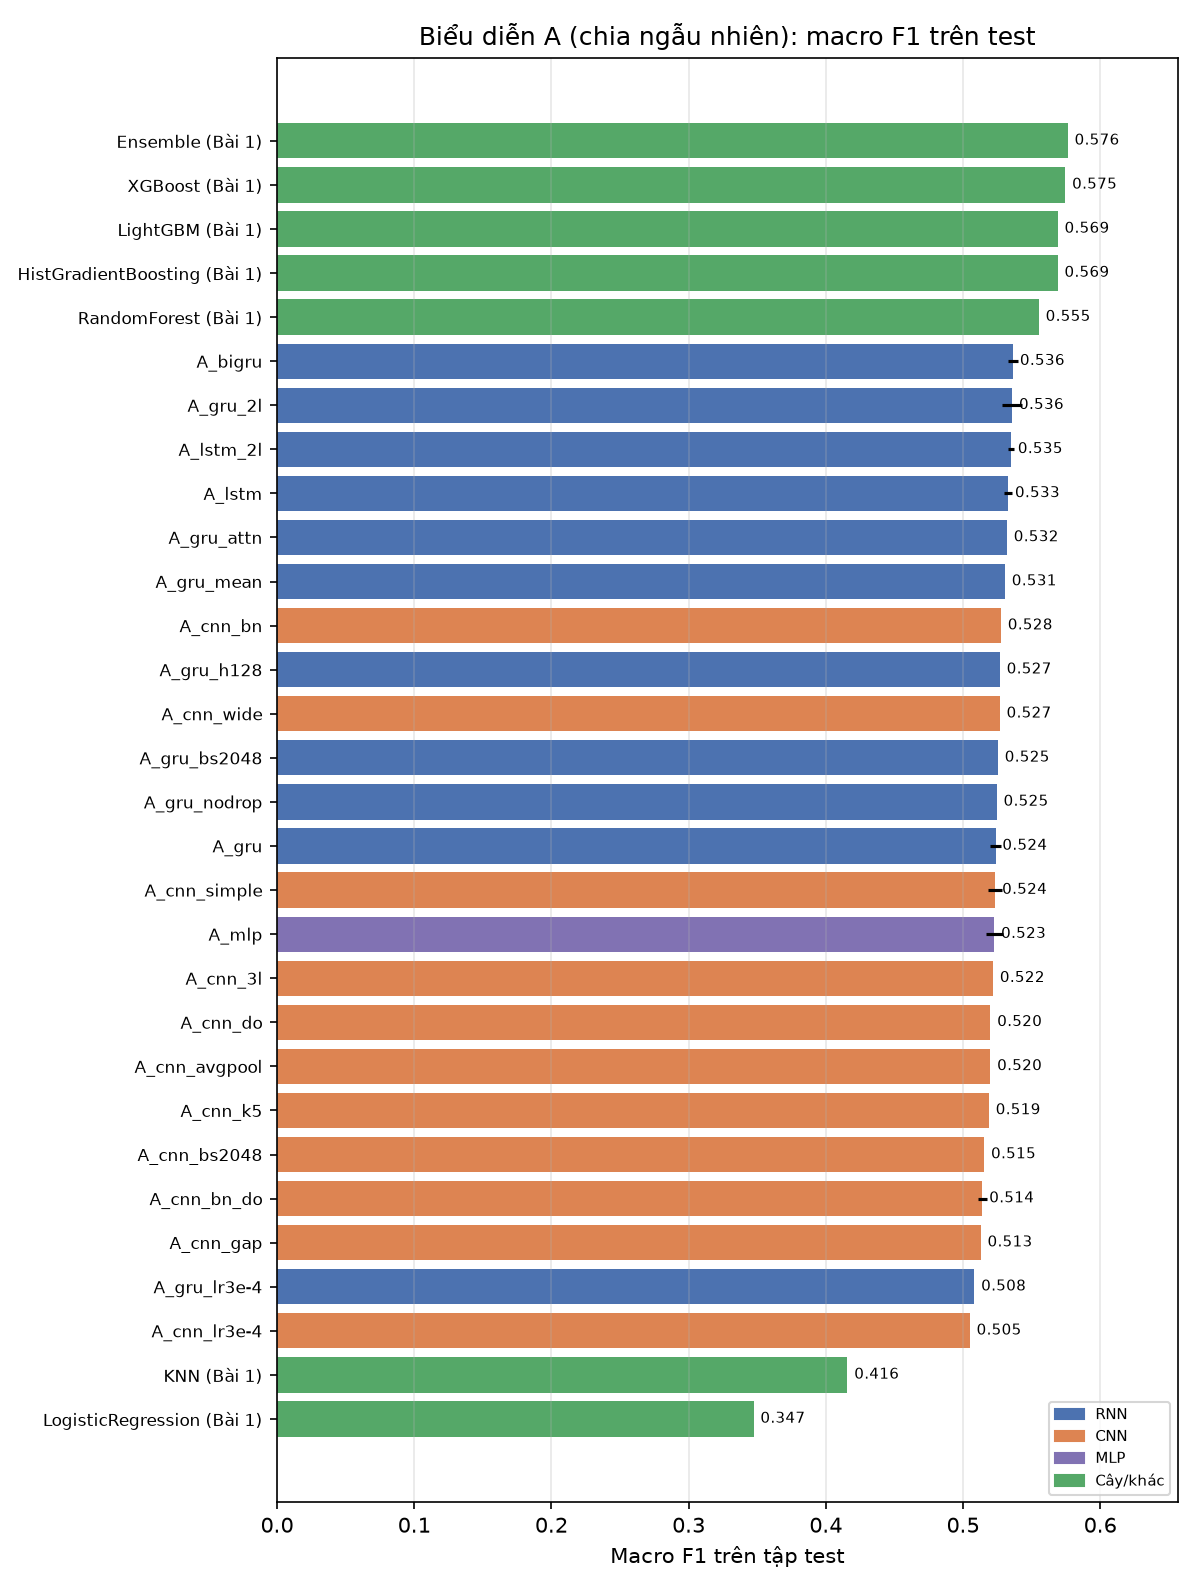
\includegraphics[height=0.78\textheight]{bars_A.png}
\column{0.48\textwidth}
\begin{itemize}\small
\item RNN 0,51--0,54; CNN 0,50--0,53; \textbf{MLP 0,52}.
\item \textbf{XGBoost Bài 1: 0,575} --- tốt hơn mọi mạng nơ-ron.
\item Mọi thay đổi kiến trúc: $\le$0,03, phần lớn trong dao động seed.
\item Xếp đặc trưng thành chuỗi \alert{không tạo thông tin mới}.
\end{itemize}
\end{columns}
\end{frame}

\begin{frame}{Kết quả biểu diễn B: +0,2 macro F1}
\begin{columns}[c]
\column{0.5\textwidth}
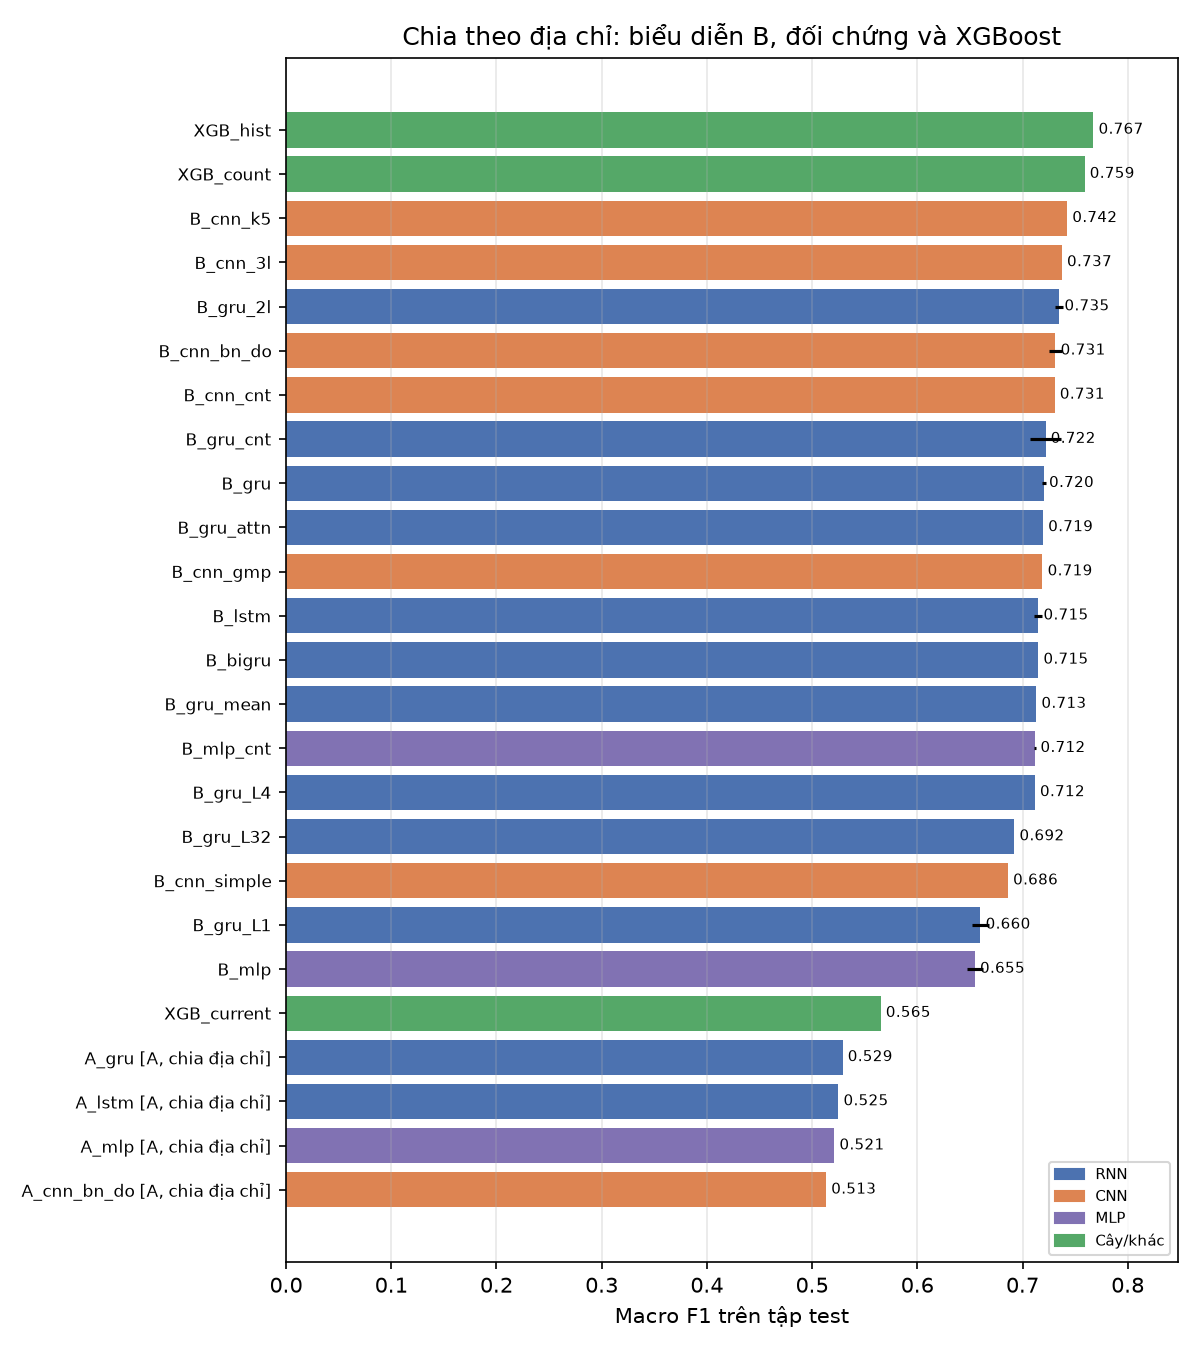
\includegraphics[height=0.78\textheight]{bars_B.png}
\column{0.48\textwidth}
\begin{itemize}\small
\item A (chia địa chỉ) $\approx$0,53 $\to$ \textbf{B 0,72--0,74}.
\item Tốt nhất: \textbf{CNN k5 0,742}; RNN: GRU 2 tầng 0,735.
\item $L=1$: 0,660 · $L=4$: 0,712 · $L=16$: 0,720 · $L=32$: 0,692.
\item \textbf{XGBoost + lịch sử tổng hợp: 0,767} --- tốt nhất.
\end{itemize}
\end{columns}
\end{frame}

\begin{frame}{RNN/CNN thắng ở địa chỉ có lịch sử dài, thua ở địa chỉ mới}
\centering\small
F1 nhị phân trên test theo số lần địa chỉ đã xuất hiện\\[4pt]
\begin{tabular}{lrrrrr}
\toprule
Số lần xuất hiện & 1 & 2 & 3--5 & 6--15 & $>$15 \\
\% dòng test & 90,3 & 3,3 & 2,9 & 2,2 & 1,2 \\
\midrule
XGBoost, không lịch sử & 0,504 & 0,469 & 0,540 & 0,524 & 0,414 \\
GRU (B) & 0,549 & 0,610 & 0,796 & 0,917 & \textbf{0,973} \\
CNN k5 (B) & 0,547 & 0,625 & \textbf{0,812} & \textbf{0,943} & 0,948 \\
XGBoost + lịch sử & \textbf{0,648} & \textbf{0,692} & 0,793 & 0,885 & 0,937 \\
\bottomrule
\end{tabular}
\vspace{6pt}
\begin{itemize}\small
\item Chuỗi giữ được \emph{chi tiết từng lần xuất hiện} mà mean/max thủ công làm mất.
\item Địa chỉ mới (90\% dòng, 53\% ransomware): mô hình cây khai thác dòng hiện tại tốt hơn.
\end{itemize}
\end{frame}

\begin{frame}{F1 từng lớp và lỗi}
\begin{columns}[c]
\column{0.42\textwidth}
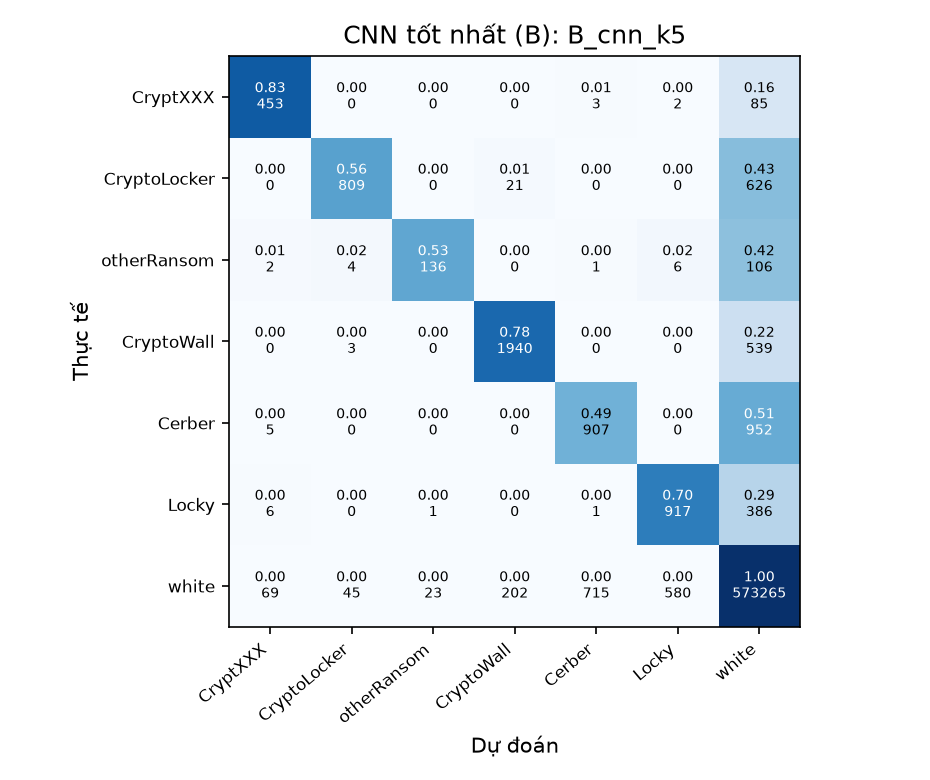
\includegraphics[width=\linewidth]{cm_B_group_B_cnn_k5.png}
\column{0.56\textwidth}
\begin{itemize}\small
\item Lịch sử giúp các họ dùng lại địa chỉ:\\ CryptoLocker 0,26$\to$0,70 · CryptoWall 0,38$\to$0,84 · otherRansom 0,08$\to$0,66.
\item Cerber/Locky (địa chỉ dùng 1 lần): không cải thiện, XGBoost tốt hơn.
\item Lỗi gần như toàn bộ là \textbf{ransomware ↔ white}; nhầm giữa các họ rất hiếm (55/7.911).
\item 78\% ransomware bị bỏ sót là địa chỉ lần đầu; với CryptoLocker/CryptoWall lần đầu, recall của mạng nơ-ron $\approx$0.
\end{itemize}
\end{columns}
\end{frame}

\begin{frame}{Overfitting / underfitting}
\begin{columns}[c]
\column{0.55\textwidth}
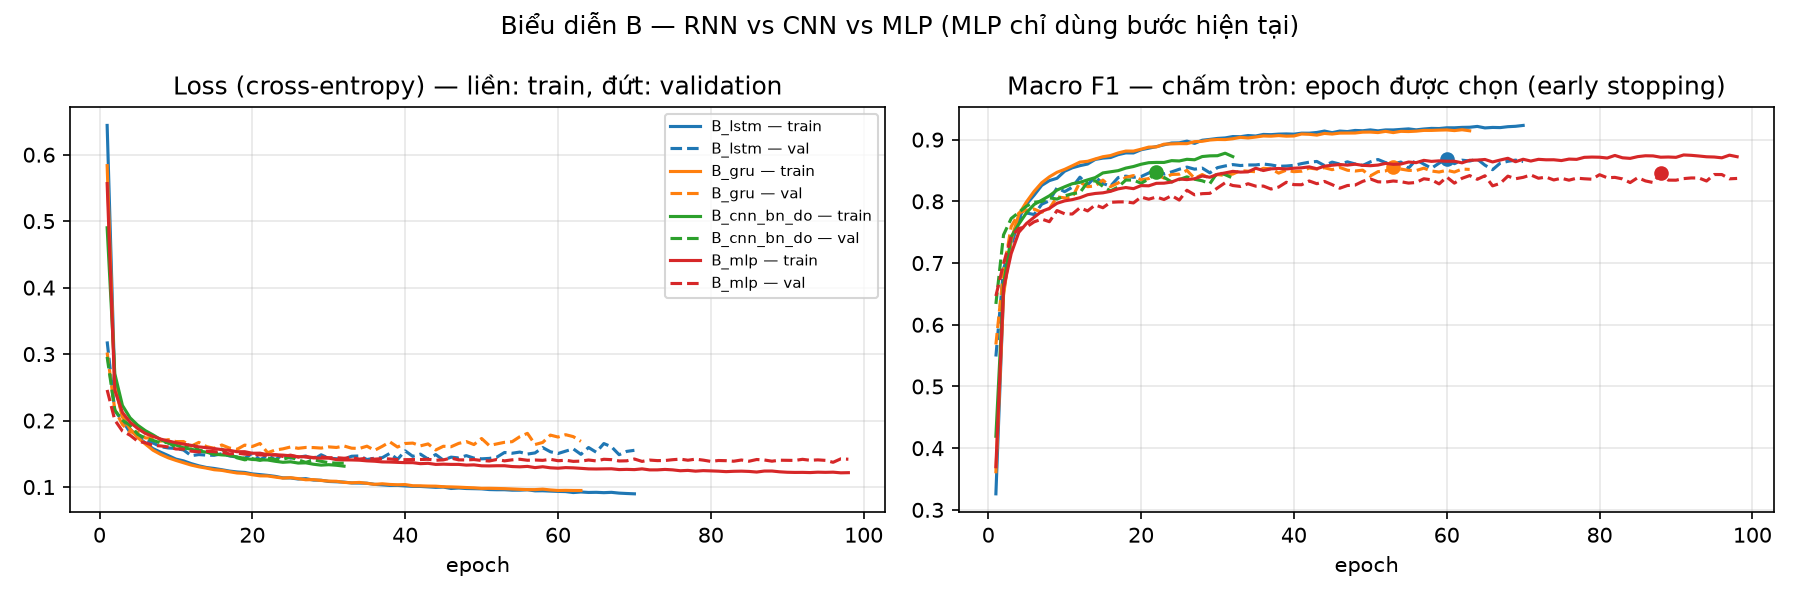
\includegraphics[width=\linewidth]{curves_B.png}
\column{0.43\textwidth}
\begin{itemize}\small
\item \textbf{A}: chênh train--val $\le$0,02; mô hình lớn hơn không giúp $\to$ giới hạn do \emph{thông tin}. Dropout/BN+DO $\to$ underfit nhẹ.
  lr $3\cdot10^{-4}$, batch 2048: chưa hội tụ.
\item \textbf{B}: F1 train 0,91 vs val 0,86; val loss tăng từ epoch $\approx$22 $\to$ overfit.
\item CNN không điều chuẩn: dừng ở epoch 12, test 0,686; \textbf{+BN+Dropout: 0,731}.
\item Biện pháp: early stopping, dropout, BN; đề xuất weight decay, label smoothing.
\end{itemize}
\end{columns}
\end{frame}

\begin{frame}{Tốc độ huấn luyện (đo riêng, giây/epoch)}
\centering\small
\begin{tabular}{lrr@{\hspace{2.5em}}lrr}
\toprule
A & Tham số & s/epoch & B & Tham số & s/epoch \\
\midrule
MLP & 22.407 & 0,29 & MLP & 22.663 & 0,33 \\
GRU 1×64 & 22.439 & 0,39 & CNN BN+DO & 16.295 & 0,68 \\
LSTM 1×64 & 27.687 & 0,41 & CNN 3 lớp & 45.351 & 0,77 \\
CNN đơn giản & 22.663 & 0,43 & GRU 1×64 & 25.607 & 0,89 \\
Bi-GRU & 42.279 & 0,48 & LSTM 1×64 & 31.879 & 0,92 \\
LSTM 2 tầng & 60.967 & 0,65 & Bi-GRU & 48.519 & 2,14 \\
\bottomrule
\end{tabular}
\vspace{6pt}
\begin{itemize}\small
\item Chuỗi ngắn cố định (A): RNN 1 tầng $\approx$ CNN. Chuỗi dài, độ dài thay đổi (B): CNN nhanh hơn RNN $\approx$25\%.
\item GRU ít tham số và nhanh hơn LSTM một chút; Bi-RNN đắt nhất mà không tốt hơn.
\end{itemize}
\end{frame}

\begin{frame}{Kết luận}
\begin{itemize}
\item \textbf{Thông tin đầu vào quan trọng hơn kiến trúc}: lịch sử địa chỉ +0,2 macro F1; đổi kiến trúc $\le$0,03.
\item Mạng nơ-ron tốt nhất: \textbf{CNN 1 chiều trên lịch sử địa chỉ} (0,742) --- vừa tốt nhất vừa nhanh nhất trong RNN/CNN.
\item Trung thực: với dữ liệu bảng, \textbf{XGBoost vẫn mạnh nhất} (0,575 ở A; 0,767 với đặc trưng lịch sử).
  RNN/CNN chỉ vượt trội khi có \emph{chuỗi thật và đủ dài}.
\item Hạn chế: \code{white} được lấy mẫu 1.000 dòng/ngày (tín hiệu lặp lại có thể lạc quan); 3 seed; một cách chia.
\item Hướng tiếp: kết hợp XGBoost (dòng hiện tại) + CNN (lịch sử), GNN trên đồ thị giao dịch, đánh giá theo thời gian.
\end{itemize}
\end{frame}

\begin{frame}[standout]
Cảm ơn thầy/cô và các bạn!\\[6pt]
\normalsize Mã nguồn: \code{final/} · Notebook: \code{final\_project.ipynb} · Báo cáo: \code{report/main.pdf}
\end{frame}

\end{document}
